\epi{``In Go, the code does exactly what it says on the page.''}{\textit{Go
Nuts mailing list}\\\textsc{ANDREW GERRAND}}
\noindent{}There are a few things that make Go different from other
languages.
\begin{description}
\item[Clean and Simple]
Go strives to keep things small and beautiful. You should
be able to do a lot in only a few lines of code;
\item[Concurrent]
Go makes it easy to ``fire off'' functions to be
run as \emph{very} lightweight threads. These threads are called
\first{goroutines}{goroutines} \footnote{Yes, that sounds a lot like
\emph{co}routines, but goroutines are slightly different as we will
see in chapter \ref{chap:channels}.} in Go;
%% gofix.go:11: non-declaration statement outside function body
\item[Channels] 
Communication with these goroutines is done
via \first{channels}{channels} \cite{csp, hoare};

\item[Fast]
Compilation is fast and execution is fast. The aim is
to be as fast as C. Compilation time is measured in seconds;

\item[Safe]
Explicit casting and strict rules when converting one type to another.
Go has garbage collection, no more \func{free()} in Go, the language takes care of this;

\item[Standard format]
A Go program can be formatted in (almost) any way the programmers want,
but an official format exists. The rule is very simple:
The output of the filter \prog{gofmt} \emph{is the officially endorsed
format}.

\item[Postfix types]
Types are given \emph{after} the variable name, thus \prog{var a int},
instead of \prog{int a;} as one would in C;

\item[UTF-8]
UTF-8 is everywhere, in strings
\emph{and} in the program code. Finally you can use \prog{$\Phi$ =
$\Phi$ + 1} in your source code;

\item[Open Source]
The Go license is completely open source, see the file LICENSE in the Go
source code distribution;

\item[Fun]
Programming with Go should be fun!

\end{description}
Erlang \cite{erlang} also shares some
of the features of Go. Notable differences between Erlang
and Go is that Erlang borders on being a functional language,
where Go is an imperative one. And Erlang runs in a virtual
machine, while Go is compiled. Go also has a much more Unix-like
feel to it.

\section{Hello World}
\label{sec:hello world}
In the Go tutorial, Go is presented to the world in the typical
manner: letting it print ``Hello World'' (Ken Thompson and
Dennis Ritchie started this when they presented the C language in 
the 1970s). We don't think we can do better, so
here it is, ``Hello World'' in Go.

\lstinputlisting[numbers=right,label=src:hello,caption=Hello world]{src/helloworld.go}
Lets look at the program line by line.
\showremarks

\section{Compiling and running code}
\label{sec:building a program}
The preferred way to build a Go program is to use the \prog{go} tool.\index{tooling!go}
To build \prog{helloworld} we just enter:
\begin{display}
\pr \user{go build helloworld.go}
\end{display}
\index{tooling!go!build}
This results in an executable called \prog{helloworld}.

\begin{display}
\pr \user{./helloworld}
\end{display}
\vspace{-3.0ex}
\texttt{Hello, world; or }%
\begin{math}\kappa\alpha\lambda\eta\mu\acute{\epsilon}\rho\alpha\hspace{1em}\kappa\end{math}%
\'o\begin{math} \sigma\mu\epsilon\end{math}\texttt{; or }こんにちは 世界
\ \newline
\ \newline

\section{Settings used in this book}
\label{sec:settings_used}
\begin{itemize}                            
\item Go itself is installed in \file{\~{}/go}, and \var{\$GOROOT} is set to \var{GOROOT=\~{}/go} ;     
\item Go source code we want to compile ourself is placed in \file{\~{}/g/src} and
\var{\$GOPATH} is set to \var{GOPATH=\~{}/g} . This variable comes into play
when we start using packages (chapter \ref{chap:packages}).
\end{itemize}

\section{Variables, types and keywords}
\label{sec:vars}
In the next few sections we will look at the variables, basic types,
keywords and control structures of our new language. 
Go has a C-like feel when it comes to its syntax. 
If you want to put two (or more) statements on one line, they must be
separated with a semicolon (';'). Normally you don't need the semicolon.

Go is different from other languages in that the type of a variable
is specified \emph{after} the variable name. So not: 
\lstinline{int a}, but \lstinline{a int}. When declaring a variable it
is assigned the ``natural'' null value for the type. This means that after
\lstinline{var a int}, \lstinline{a} has a value of 0. With
\lstinline{var s string}, \lstinline{s} is assigned the zero string,
which is \lstinline{""}. 

Declaring and assigning in Go is a two step process, but they may
be combined. Compare the following pieces of code which have
the same effect. 
\index{variables!declaring}
\index{variables!assigning}

\begin{minipage}{.5\textwidth}
\begin{lstlisting}[linewidth=.5\textwidth,caption={Declaration with =}]
var a int
var b bool
a = 15
b = false
\end{lstlisting}
\hfill
\end{minipage}
\begin{minipage}{.5\textwidth}
\begin{lstlisting}[linewidth=.5\textwidth,caption={Declaration with :=}]
a := 15
b := false
\end{lstlisting}
\ \\
\ \\
\hfill
\end{minipage}

On the left we use the
\key{var} keyword to declare a variable and \emph{then} assign a value to
it. The code on the right uses \mbox{\key{:=}{ }} to do this in one
step (this form may only be used \emph{inside} functions).
In that case the variable
type is \emph{deduced} from the value. A value of 15 indicates an \type{int},
a value of \texttt{false} tells Go that the type should be \type{bool}. 
Multiple \key{var} declarations may also be grouped; \key{const}
and \key{import} also allow this. Note the use of parentheses:
\begin{lstlisting}
var (
    x int
    b bool
)
\end{lstlisting}
Multiple variables of the same type can also be declared on a
single line: \lstinline{var x, y int} makes \var{x} and \var{y} both
\type{int} variables. You can also make use of \first{parallel
assignment}{parallel assignment}:
\begin{lstlisting}
a, b := 20, 16
\end{lstlisting}
Which makes \var{a} and \var{b} both integer variables and assigns
20 to \var{a} and 16 to \var{b}.

A special name for a variable is \var{\textbf{\_}} \index{variables!\_}
(underscore)\index{variables!underscore}. Any value
assigned to it is discarded. In this example we only assign the integer
value of 35 to \var{b} and discard the value 34.
\begin{lstlisting}
_, b := 34, 35
\end{lstlisting}
Declared but otherwise unused variables are a compiler error in Go. The
following code generates this error:
\error{i declared and not used}

\begin{lstlisting}
package main
func main() { 
    var i int
}
\end{lstlisting}

\subsection{Boolean types}
A boolean type represents the set of boolean truth values denoted by the
predeclared constants \emph{true} and \emph{false}. The boolean type is \type{bool}.

\subsection{Numerical types}
Go has the well known types such as \lstinline{int}. This type
has the appropriate length for your machine,
meaning that on a 32-bit machine it is 32 bits and on
a 64-bit machine it is 64 bits. Note: an \lstinline{int} is
either 32 or 64 bits, no other values are defined. Same goes 
for \lstinline{uint}.

If you want to be explicit about the length you can have
that too with \lstinline{int32}, or \lstinline{uint32}. The full
list for (signed and unsigned) integers is
\type{int8}, \type{int16}, \type{int32}, \type{int64} and
\type{byte}, \type{uint8}, \type{uint16}, \type{uint32}, \type{uint64}.
With \lstinline{byte} being an
alias for \lstinline{uint8}. For floating point values there is
\lstinline{float32} and \lstinline{float64} (there is no \lstinline{float} type). 
A 64 bit integer or floating point value is \emph{always} 64 bit, also on 32 bit
architectures.

Note however
that these types are all distinct and assigning variables which mix
these types is a compiler error, like in the following code:
\lstinputlisting[numbers=right,label=src:types,caption=Familiar types are still distinct]{src/types.go}
Gives the error on the assignment on line 7:

\noindent\error{types.go:7: cannot use a + a (type int)  as type int32 in assignment}

The assigned values may be denoted using octal, hexadecimal or the scientific notation:
\lstinline{077}, \lstinline{0xFF}, \lstinline{1e3} or
\mbox{\lstinline{6.022e23}} are all valid.

\subsection{Constants}
\label{sec:constants}
Constants in Go are just that --- constant. They are created at compile
time, and can only be numbers, strings or booleans;
\lstinline{const x = 42} makes \var{x} a constant. You can use
\first{\key{iota}}{keyword!iota} \footnote{The word [iota] is used in a common English phrase,
'not one iota', meaning 'not the slightest difference', in reference to
a phrase in the New Testament: ``\emph{until heaven and earth pass away, not an
iota, not a dot, will pass from the Law}.'' \cite{iota}}
to enumerate values.
\begin{lstlisting}
const (
	a = iota
	b = iota 
)
\end{lstlisting}
The first use of \key{iota} will yield 0, so \var{a} is equal to 0, whenever
\key{iota} is used again on a new line its value is incremented with 1, so \var{b}
has a value of 1.

You can even do the following, let Go repeat the use of \key{= iota}:
\begin{lstlisting}
const (
	a = iota
	b	    |\coderemark{Implicitly \texttt{b = iota}}|
)
\end{lstlisting}
You may also explicitly type a constant, if you need that:
\begin{lstlisting}
const (
	a = 0           |\coderemark{Is an \key{int} now}|
	b string = "0" 
)
\end{lstlisting}

\subsection{Strings}
Another important built-in type is \lstinline{string}. Assigning a
string is as simple as:
\begin{lstlisting}
s := "Hello World!"
\end{lstlisting}
Strings in Go are a sequence of UTF-8 characters enclosed in double
quotes ("). If you use the single quote (') you mean one character
(encoded in UTF-8) --- which is \emph{not} a \lstinline{string} in Go.

Once assigned to a variable the string can not be changed: strings in Go are
immutable. For
people coming from C, the following is not legal in Go:
\begin{lstlisting}
var s string = "hello"
s[0] = 'c'  |\coderemark{Change first char. to 'c', this is an error}|
\end{lstlisting}
To do this in Go you will need the following:
\begin{lstlisting}
s := "hello"
c := []rune(s)	    |\longremark{Convert \var{s} to an array of runes, see %
chapter \ref{chap:beyond} section ``\titleref{sec:conversions}'' on %
page \pageref{sec:conversions};}|
c[0] = 'c'	    |\longremark{Change the first element of this %
array;}|
s2 := string(c)     |\longremark{Create a \emph{new} %
string \var{s2} with the alteration;}|
fmt.Printf("%s\n", s2) |\longremark{print the string with \func{fmt.Printf}.}|
\end{lstlisting}
\showremarks

\begin{lbar}[Multi-line strings]
Due to the insertion of semicolons (see \cite{effective_go} section
``Semicolons''), you need to be careful with using multi line strings. If
you write:
\begin{lstlisting}
s := "Starting part"
    + "Ending part"
\end{lstlisting}
This is transformed into:
\begin{lstlisting}
s := "Starting part";
    + "Ending part";
\end{lstlisting}
Which is not valid syntax, you need to write:
\begin{lstlisting}
s := "Starting part" +
     "Ending part"
\end{lstlisting}
Then Go will not insert the semicolons in the wrong places. Another way
would be to use \emph{raw} string literals\index{string literal!raw} by using backquotes (\key{`}):
\begin{lstlisting}
s := `Starting part
     Ending part`
\end{lstlisting}
Be aware that in this last example \var{s} now also contains the newline.
Unlike \emph{interpreted} string literals \index{string literal!interpreted} the value of a raw string literal
is composed of the \emph{uninterpreted} characters between the quotes.
\end{lbar}

\subsection{Runes}
\lstinline{Rune} is an alias for int32. It is an UTF-8 encoded code point. When is this type useful? For instance,
when iterating over characters in a string. You can loop over each byte (which is only equivalent to a character
when strings are encoded in 8-bit ASCII, which they are \emph{not} in Go!). So to get the actual characters you
should use the \type{rune} type.

\subsection{Complex numbers}
Go has native support for complex numbers. To
use them you need a variable of type \lstinline{complex128} (64
bit real and imaginary parts) or \lstinline{complex64} (32 bit
real and imaginary parts).
Complex numbers are written as
\var{re + im$i$}, where \var{re} is the real part,
\var{im} is the imaginary part and $i$ is the literal '$i$' ($\sqrt{-1}$).
An example of using complex numbers:

\gomarginpar{The Printf() verb \%v, means ``print the value in its default format''.}
\lstinline{var c complex64 = 5+5i; fmt.Printf("Value is: %v", c)}\newline
will print: \lstinline{(5+5i)}

\subsection{Errors}
Any non-trivial program will have the need for error reporting sooner or later. Because of this
Go has a builtin type specially for errors, called \lstinline{error}.

\lstinline{var e error} creates a variable \var{e} of type \lstinline{error} with the value \lstinline{nil}.

\section{Operators and built-in functions}
\label{sec:builtins}
Go supports the normal set of numerical operators.
Table \ref{tab:op-precedence}
lists the current ones and their relative precedence. They
all associate from left to right.

\begin{table}[H]
\begin{center}
\caption{Operator precedence}
\label{tab:op-precedence}
\begin{tabular}{ll}
\textbf{precedence} & \textbf{operator(s)} \\ \hline
highest   &	\verb!*  /  %  <<  >>  &  &^!		\\
    &	\verb!+  -  | ^!			\\
    &	\verb+==  !=  <  <=  >  >=+		\\
    &	\verb!<-!				\\
    &	\verb!&&!				\\
lowest    &	\verb!||!				\\
\end{tabular}

\end{center}
\end{table}
\verb|+ - * /| and \verb|%| all do what you would expect,
\verb!& | ^!
and \verb!&^! are bit operators for
\first{bitwise and}{operator!bitwise!and}, 
\first{bitwise or}{operator!bitwise!or}, \first{bitwise xor}{operator!bit
wise xor} and \first{bit clear}{operator!bitwise!clear} respectively.
The \verb|&&| and \verb/||/ operators are 
logical \first{and}{operator!and} and
logical \first{or}{operator!or}. Not listed in the table
is the logical \first{not}{operator!not}: \verb/!/

Although Go does not support operator overloading (or method
overloading for that matter), some of the built-in
operators \emph{are} overloaded. For instance, \texttt{+} can be used for integers,
floats, complex numbers and strings (adding strings is concatenating
them). 

\section{Go keywords}
\begin{table}[H]
\begin{center}
\caption{Keywords in Go}
\label{tab:keywords}
%%%%%%%%%%%%%%%%%%%%%%%%%%%%%%%%%%%%%%%%%%%%%%%%%%%%%%%%%%%%%%%%%%%%%%
%%                                                                  %%
%%  This is a LaTeX2e table fragment exported from Gnumeric.        %%
%%                                                                  %%
%%%%%%%%%%%%%%%%%%%%%%%%%%%%%%%%%%%%%%%%%%%%%%%%%%%%%%%%%%%%%%%%%%%%%%
\begin{tabular}{lllll}
\key{break}	&\key{default}          &\key{for}	&\key{import}    &\key{return}\\
\key{case}	&\key{defer}            &\key{func}	&\key{interface}          &\key{select}\\
\key{chan}	&\key{delete}           &\key{go}	&\key{map}      &\key{struct}\\
\key{const}	&\key{else}    	    &\key{goto}	&\key{package}        &\key{switch}\\
\key{continue}	&\key{fallthrough}      &\key{if}	&\key{range}       &\key{type}\\
               &                       &               &                   &\key{var}\\
\end{tabular}

\end{center}
\end{table}
Table \ref{tab:keywords} lists all the keywords in Go. 
We will cover them in the following paragraphs and chapters. Some
of them we have seen already.
\begin{itemize}
\item For \key{var} and \key{const} see ``\titleref{sec:vars}'' on
page \pageref{sec:vars};
\item \key{package} and \key{import} are briefly touched on in section ``\titleref{sec:hello world}''.
In chapter \ref{chap:packages} they are documented in more detail.
\end{itemize}
Others deserve more text and have their own chapter/section:
\begin{itemize}
\item \key{func} is used to declare functions and methods;
\item \key{return} is used to return from functions, for both \key{func}
and \key{return} see chapter \ref{chap:functions} for the details;
\item \key{go} is used for concurrency, see chapter \ref{chap:channels};
\item \key{select} used to choose from different types of communication, see chapter \ref{chap:channels};
\item \key{interface} see chapter \ref{chap:interfaces};
\item \key{struct} is used for abstract data types, see chapter \ref{chap:beyond};
\item \key{type} also see chapter \ref{chap:beyond}.
\end{itemize}

\section{Control structures}
There are only a few control structures in 
Go \footnote{This section is copied from \cite{effective_go}.}.
For instance there is no do or while loop, only a 
\key{for}. There is a (flexible) \key{switch} statement and \key{if} and
\key{switch} accept an
optional initialization statement like that of \key{for}. There also is
something called a type switch and a multiway communications
multiplexer, \key{select} (see chapter \ref{chap:channels}). The syntax is 
different (from that in C): parentheses
are not required and the body must \emph{always} be brace-delimited.

\subsection{If-else}
In Go an \first{\key{if}}{keyword!if} looks like this:
\begin{lstlisting}
if x > 0 {	|\coderemark{\{ is mandatory}|
    return y
} else {
    return x
}
\end{lstlisting}
Mandatory braces encourage writing simple \key{if} statements on multiple
lines. It is good style to do so anyway, especially when the body
contains a control statement such as a
\first{\key{return}}{keyword!return} or
\first{\key{break}}{keyword!break}.

Since \key{if} and \key{switch} accept an initialization statement, it's common to
see one used to set up a (local) variable.
\begin{lstlisting}
if err := file.Chmod(0664); err != nil {  |\coderemark{\texttt{nil} is %
like C's NULL}|
    fmt.Printf(err) |\coderemark{Scope of \var{err} is limited to %
\key{if}'s body}|
    return err
}
\end{lstlisting}
You can use the logical operators (see table \ref{tab:op-precedence}) as
you would normally:
\begin{lstlisting}
if true && true  {
    fmt.Println("true")
}
if ! false {
    fmt.Println("true")
}
\end{lstlisting}

In the Go libraries, you will find that when an \key{if} statement doesn't flow
into the next statement -- that is, the body ends in \key{break},
\key{continue}, \key{goto},
or \key{return} -- the unnecessary \first{\key{else}}{keyword!else} is omitted.

\begin{lstlisting}
f, err := os.Open(name, os.O_RDONLY, 0)
if err != nil {
    return err
}
doSomething(f)
\end{lstlisting}
This is an example of a common situation where code must analyze a
sequence of error possibilities. The code reads well if the successful
flow of control runs down the page, eliminating error cases as they
arise. Since error cases tend to end in \key{return} statements, the resulting
code needs no \key{else} statements.
\begin{lstlisting}
f, err := os.Open(name, os.O_RDONLY, 0)
if err != nil {
    return err
}
d, err := f.Stat()
if err != nil {
    return err
}
doSomething(f, d)
\end{lstlisting}
Syntax-wise the following is illegal in Go:
\begin{lstlisting}
if err != nil
{		    |\coderemark{Must be on the same line as the if}|
    return err
}
\end{lstlisting}
See \cite{effective_go} section ``Semicolons'' for the deeper reasons
behind this.

\begin{lbar}[Ending with \key{if-then-else}]
Note that if you end a function like this:
\begin{lstlisting}
if err != nil {
    return err
} else {
    return nil
}
\end{lstlisting}
It will not compile. This is a bug in the Go compiler. See
\cite{go_issue_65} for an extended problem description and
hopefully a fix.
\end{lbar}

\subsection{Goto}
Go has a \first{\key{goto}}{keyword!goto} statement --- use it wisely. With \key{goto}
you jump to a \index{label} label which must be defined within the current function.
For instance, a loop in disguise:
\begin{lstlisting}
func myfunc() {
        i := 0                                                                                      
Here:	   |\coderemark{First word on a line ending with a colon is a label}|
        println(i)
        i++ 
        goto Here |\coderemark{Jump}|
}
\end{lstlisting}
The name of the label is case sensitive.

\subsection{For}
\label{sec:for}
The Go \first{\key{for}}{keyword!for} loop has three forms, only one of
which has semicolons.
\begin{lstlisting}
for init; condition; post { } |\coderemark{Like a C \key{for}}|

for condition { }             |\coderemark{Like a while}|

for { }                       |\coderemark{ Like a C \key{for(;;)} (endless loop)}|
\end{lstlisting}
Short declarations make it easy to declare the index variable right in the loop.
\begin{lstlisting}
sum := 0
for i := 0; i < 10; i++ {
    sum += i	|\coderemark{Short for sum = sum + i}|
}   |\coderemark{\var{i} ceases to exist \emph{after} the loop}|
\end{lstlisting}
Finally, since Go has no comma operator and ++ and - - are statements not
expressions, if you want to run multiple variables in a \key{for} you should
use \first{parallel assignment}{parallel assignment}.
\begin{lstlisting}
// Reverse a
for i, j := 0, len(a)-1; i < j; i, j = i+1, j-1 { |\coderemark{Parallel assignment}|
    a[i], a[j] = a[j], a[i] |\coderemark{Here too}|
}
\end{lstlisting}

\subsection{Break and continue}
With \first{\key{break}}{keyword!break} you can quit loops early.  By itself, \key{break} breaks
the current loop.
\begin{lstlisting}
for i := 0; i < 10; i++ {
    if i > 5 {
	break |\coderemark{Stop this loop, making it only print 0 to 5}|
    }
    println(i)
}
\end{lstlisting}
With loops within loops you can specify a label after \key{break}.
Making the label identify \emph{which} loop to stop:
\begin{lstlisting}
J:  for j := 0; j < 5; j++ {
	for i := 0; i < 10; i++ {
	    if i > 5 { 
		break J	|\coderemark{Now it breaks the \var{j}-loop, not the \var{i} one}|
	    }
	    println(i)
	}
    } 
\end{lstlisting}

With \first{\key{continue}}{keyword!continue} you begin the next iteration of the
loop, skipping any remaining code. In the same way as \key{break},
\key{continue} also accepts a label. The following loop prints 0 to 5.
\begin{lstlisting}
for i := 0; i < 10; i++ {
    if i > 5 {
	continue |\coderemark{Skip the rest of the remaining code in the loop}|
    }
    println(i)
}
\end{lstlisting}

\subsection{Range}
The keyword \first{\key{range}}{keyword!range} can be used for loops. It
can loop over slices, arrays, strings, maps and channels (see chapter
\ref{chap:channels}). \key{range} is
an iterator that, when called, returns the next key-value pair from the thing it
loops over. Depending on what that is, \key{range} returns
different things.

When looping over a slice or array \key{range} returns the index in the
slice as the key and value belonging to that index.
Consider this code: \index{keyword!range!on slices}
\begin{lstlisting}
list := []string{"a", "b", "c", "d", "e", "f"}     |\longremark{Create a %
slice (see ``\titleref{sec:arrays}'' on page \pageref{sec:arrays}) of strings.}|
for k, v := range list {	|\longremark{Use \key{range} to loop over them. %
With each iteration \key{range} will return the index as an \type{int} and %
the key as a \type{string}, starting with 0 and ``a''.}|
    // do what you want with k and v \longremark{\var{k} will have the value 0\ldots5, and %
\var{v} will loop through ``a''\ldots``f''.}
}
\end{lstlisting}
\showremarks

You can also use \key{range} on strings directly. Then it
will break out the individual Unicode characters 
\footnote{In the UTF-8 world characters are sometimes called \first{runes}{runes}. 
Mostly, when people talk about
characters, they mean 8 bit characters. As UTF-8 characters may be up to 32 bits the word
rune is used. In this case the type of \var{char} is \type{rune}.} and their start position, by parsing the UTF-8.
The loop: \index{keyword!range!on maps}
\begin{lstlisting}
for pos, char := range "a|$\Phi{}$|x" {
    fmt.Printf("character '%c' starts at byte position %d\n", char, pos)
}
\end{lstlisting}
prints
\begin{display}
character 'a' starts at byte position 0
character '\begin{math}\Phi\end{math}' starts at byte position 1
character 'x' starts at byte position 3 \coderemark{\begin{math}\Phi\end{math} took 2 bytes}
\end{display}

\subsection{Switch}
Go's \first{\key{switch}}{keyword!switch} is very flexible. The expressions need
not be
constants or even integers; the cases are evaluated top to bottom until
a match is found, and if the \key{switch} has no expression it switches on
\type{true}. It's therefore possible -- and idiomatic -- to write an
\key{if-else-if-else} chain as a \key{switch}.
\begin{lstlisting}
func unhex(c byte) byte {
    switch {
    case '0' <= c && c <= '9':
        return c - '0'
    case 'a' <= c && c <= 'f':
        return c - 'a' + 10
    case 'A' <= c && c <= 'F':
        return c - 'A' + 10
    }
    return 0
}
\end{lstlisting}
There is no automatic fall through, you can however use
\first{\key{fallthrough}}{keyword!fallthrough} to do just that.
Without \key{fallthrough}:
\begin{lstlisting}
switch i {
    case 0:  // empty case body
    case 1:
	f()  // f is not called when i == 0!
}
\end{lstlisting}
And with:
\begin{lstlisting}
switch i {
    case 0:  fallthrough
    case 1:
	f()  // f is called when i == 0!
}
\end{lstlisting}
With \first{\key{default}}{keyword!default} you can specify an action
when none of the other cases match.
\begin{lstlisting}
switch i {
    case 0:  
    case 1:
	f()
    default:	
	g()	// called when i is not 0 or 1
}
\end{lstlisting}
Cases can be presented in comma-separated lists.
\begin{lstlisting}
func shouldEscape(c byte) bool {
    switch c {
    case ' ', '?', '&', '=', '#', '+': |\coderemark{, as "or"}|
        return true
    }
    return false
}
\end{lstlisting}
Here's a comparison routine for byte arrays that uses two \key{switch} statements:
\begin{lstlisting}
// Compare returns an integer comparing the two byte arrays
// lexicographically.
// The result will be 0 if a == b, -1 if a < b, and +1 if a > b
func Compare(a, b []byte) int {
    for i := 0; i < len(a) && i < len(b); i++ {
        switch {
        case a[i] > b[i]:
            return 1
        case a[i] < b[i]:
            return -1
        }
    }
    // Strings are equal except for possible tail
    switch {
    case len(a) < len(b):
        return -1
    case len(a) > len(b):
        return 1
    }
    return 0	// Strings are equal
}
\end{lstlisting}

\section{Built-in functions}
A small number of functions are predefined, meaning 
you \emph{don't} have to include any package to get
access to them. Table \ref{tab:predef-functions} lists them all.\footnote{You can use the
command \prog{go doc builtin} to read the online documentation about the built-in types and functions.}

\begin{table}[H]
\begin{center}
\caption{Pre--defined functions in Go}
\label{tab:predef-functions}
\begin{tabular}{lllll}
\key{close}	&\key{new}	&\key{panic}	&\key{complex} \\
\key{delete}   &\key{make}     &\key{recover}  &\key{real} \\
\key{len}	&\key{append}	&\key{print}	&\key{imag}  \\
\key{cap}	&\key{copy}	&\key{println}	&\\
\end{tabular}

\end{center}
\end{table}

These built-in functions are documented in the \package{builtin} \index{package!builtin}
pseudo package that is included in recent Go releases.

\paragraph{\func{close}} is used in
channel communication. It closes a channels, see chapter \ref{chap:channels}
for more on this.
\index{built-in!close}

\paragraph{\func{delete}} is used for deleting entries in maps.
\index{built-in!delete}

\paragraph{\func{len} and \func{cap}} are used on a number of different
types, \func{len} is
used for returning the length of strings and the length of slices and
arrays. See section ``\titleref{sec:arrays}'' for the details of slices and
arrays and the function
\func{cap}.\index{built-in!len}\index{built-in!cap}

\paragraph{\func{new}} is used for allocating memory for user defined
data types. See section ``\titleref{sec:allocation with new}'' on page
\pageref{sec:allocation with new}.
\index{built-in!new}

\paragraph{\func{make}} is used for allocating memory for built-in
types (maps, slices and channels). See section 
``\titleref{sec:allocation with make}'' on page
\pageref{sec:allocation with make}.
\index{built-in!make}

\paragraph{\func{copy}} is used for copying slices. 
See section ``\titleref{sec:slices}'' in this chapter.
\index{built-in!copy}

\paragraph{\func{append}} is for concatenating slices. 
See section ``\titleref{sec:slices}'' in this chapter.
\index{built-in!append}

\paragraph{\func{panic} and \func{recover}} are used for an 
\emph{exception} mechanism. See the section ``\titleref{sec:panic}'' on 
page \pageref{sec:panic} for more.
\index{built-in!panic}
\index{built-in!recover}

\paragraph{\func{print} and \func{println}} are low level printing
functions that can be used without reverting to the
\package{fmt}\index{package!fmt}
package. These are mainly used for debugging.
\index{built-in!print}\index{built-in!println}

\paragraph{\func{complex}, \func{real} and \func{imag}} all deal with
\first{complex numbers}{complex numbers}. Apart from the simple example
we gave, we will not further explain complex numbers.
\index{built-in!complex}
\index{built-in!real}
\index{built-in!imag}


\section{Arrays, slices and maps}
\label{sec:arrays}
Storing multiple values in a list can be done by utilizing arrays, or
their more flexible cousin: slices. A dictionary or hash type is also
available, it is called a \type{map} in Go.

\subsection{Arrays}
An array is defined by: \verb|[n]<type>|, where $n$ is the length
of the array and \verb|<type>| is the stuff you want to store.
Assigning or indexing an element in the array is done with square
brackets:
\begin{lstlisting}
var arr [10]int
arr[0] = 42
arr[1] = 13
fmt.Printf("The first element is %d\n", arr[0])
\end{lstlisting}
Array types like \lstinline{var arr = [10]int} have a fixed size. The
size is \emph{part} of the type.
They can't grow, because then they would have a different type. Also arrays
are values: Assigning one array to another \emph{copies} all the elements.
In particular, if you pass an array to a function it will receive a
copy of the array, not a pointer to it. 

\index{array!multidimensional}
To declare an array you can use the following: \lstinline{var a [3]int},
to initialize it to something other than zero use a
\first{composite literal}{literal!composite}: \lstinline|a := [3]int{1, 2, 3}|.
This can be shortened to \lstinline|a := [...]int{1, 2, 3}|, where Go counts
the elements automatically. \gomarginpar{A composite literal allows you
to assign a value directly to an array, slice or map.

See the section ``\titleref{sec:constructors and composite literals}'' on
page \pageref{sec:constructors and composite literals} for more.}
Note that all fields must be specified.  So if you are using multidimensional
arrays you have to do quite some typing:
\begin{lstlisting}
a := [2][2]int{ [2]int{1,2}, [2]int{3,4} }
\end{lstlisting}
Which is the same as:
\begin{lstlisting}
a := [2][2]int{ [...]int{1,2}, [...]int{3,4} }
\end{lstlisting}
When declaring arrays you \emph{always} have to type something in
between the square brackets, either a number or three dots (\verb|...|)
when using a composite literal. 
\gomarginpar{Go release \gorelease{2010-10-27} \cite{go_release_hist}.} 
Since release \gorelease{2010-10-27} this syntax was further simplified.
From the release notes:
\begin{quote}
The syntax for arrays, slices, and maps of composite literals has been
simplified. Within a composite literal of array, slice, or map type, elements
that are themselves composite literals may elide the type if it is identical to
the outer literal's element type. 
\end{quote}
This means our example can become:
\begin{lstlisting}
a := [2][2]int{ {1,2}, {3,4} }
\end{lstlisting}

\subsection{Slices}
\label{sec:slices}
\todo{Add push/pop to this section as container/vector will be deprecated.}
A slice is similar to an array, but it can grow when new elements
are added.
A slice always refers to an underlying array. What makes slices different
from
arrays is that a slice is a pointer \emph{to} an array;
slices are \first{reference types}{reference types}, 
\gomarginpar{Reference types are created with \lstinline{make}.}
which means that if you assign one slice to
another, both refer to the same underlying array. For instance, if a
function takes a slice argument, changes it makes to the elements of the
slice will be visible to the caller, analogous to passing a pointer to
the underlying array. With:
\begin{lstlisting}
sl := make([]int, 10)
\end{lstlisting}
you create a slice which can hold ten elements. Note that the
underlying array isn't specified.
A slice is always coupled to an array that has
a fixed size. For slices we define a \first{capacity}{slice!capacity} and a
\first{length}{slice!length}. \index{array!length}\index{array!capacity}
Figure \ref{fig:array-vs-slice} depicts the following Go code.
First we create an array of $m$ elements of the type \lstinline{int}:
\lstinline{var array[m]int}\newline
Next, we create a slice from this array:
\lstinline{slice := array[0:n]}\newline
And now we have:
\begin{itemize}
\item{\lstinline{len(slice) == n}{} ;}
\item{\lstinline{cap(slice) == m}{} ;}
\item{\lstinline{len(array) == cap(array) == m}{} .}
\end{itemize}
\begin{figure}[H]
\caption{Array versus slice}
\label{fig:array-vs-slice}
\begin{center}
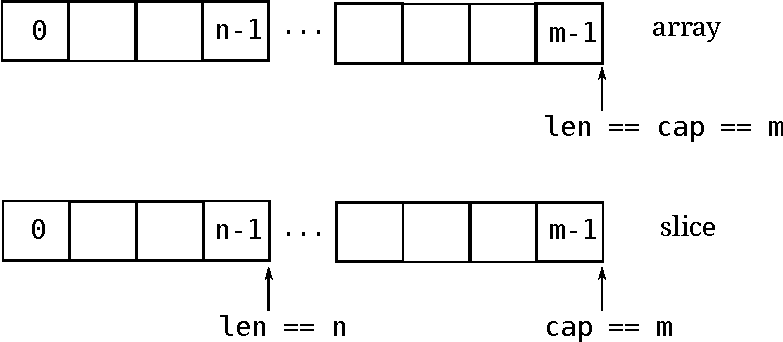
\includegraphics[scale=0.65]{fig/array-vs-slice.pdf}
\end{center}
\end{figure}

Given an array, or another slice, a new slice is created via
\lstinline{a[I:J]}. This creates a new slice which refers to 
the variable \lstinline{a}, starts at index \var{I}, and ends
before index \var{J}. It has length \lstinline{J - I}.

\begin{lstlisting}
// array[n:m], create a slice from array with elements n to m-1
a := [...]int{1, 2, 3, 4, 5} |\longremark{Define an array with 5 %
elements, from index 0 to 4;}|
s1 := a[2:4] |\longremark{Create a slice with the elements from index 2 %
to 3, this contains: \texttt{3, 4};}|
s2 := a[1:5] |\longremark{Create a slice with the elements from index 1 %
to 4, contains: \texttt{2, 3, 4, 5};}|
s3 := a[:]   |\longremark{Create a slice with all the elements of the %
array in it. This is a shorthand for: \texttt{a[0:len(a)]};}|
s4 := a[:4]  |\longremark{Create a slice with the elements from index %
0 to 3, this is thus short for: \texttt{a[0:4]}, and yields: \texttt{1, 2, %
3, 4};}|
s5 := s2[:]  |\longremark{Create a slice from the slice \var{s2}, note that %
\texttt{s5} still refers to the array \texttt{a}.}|
\end{lstlisting}
\showremarks

In the code listed in \ref{src:arrays} we dare to do the impossible on
line 8 and try to allocate something
beyond the capacity (maximum length of the underlying array) and
we are greeted with a \emph{runtime} error.
\lstinputlisting[numbers=right,label=src:arrays,caption=Arrays and slices]{src/array-and-slices.go}
If you want to extend a slice, there are a couple of built-in functions
that make life easier:
\lstinline{append} and \lstinline{copy}. From \cite{go_spec}:
\begin{quote}
The function \lstinline{append} appends zero or more values \lstinline{x} to a
slice \lstinline{s} and returns the resulting slice, with the same type as
\lstinline{s}.
If the capacity of \lstinline{s} is not large enough to fit the additional values,
\lstinline{append} allocates a new, sufficiently large slice that fits both the
existing slice elements and the additional values. Thus, the returned
slice may refer to a different underlying array.
\end{quote}
\index{built-in!append}
\begin{lstlisting}
s0 := []int{0, 0}
s1 := append(s0, 2)       |\longremark{append a single element, \texttt{s1 == []int\{0, 0, 2\}};}|
s2 := append(s1, 3, 5, 7) |\longremark{append multiple elements, %% 
\texttt{s2 == []int\{0, 0, 2, 3, 5, 7\}};}|
s3 := append(s2, s0...)   |\longremark{append a slice, \texttt{s3 == []int\{0, 0, 2, 3, 5, 7, 0, 0\}}. %%
Note the three dots!}|
\end{lstlisting}
\showremarks
And
\begin{quote}
The function \lstinline{copy} copies slice elements from a source
\lstinline{src} to a
destination \lstinline{dst} and returns the number of elements copied. Source and
destination may overlap. The number of arguments
copied is the minimum of \lstinline{len(src)} and
\mbox{\lstinline{len(dst)}}.
\end{quote}
\index{built-in!copy}
\begin{lstlisting}
var a = [...]int{0, 1, 2, 3, 4, 5, 6, 7}
var s = make([]int, 6)
n1 := copy(s, a[0:])    |\coderemark{\texttt{n1 == 6, s == []int\{0, 1, 2, 3, 4, 5\}}}|
n2 := copy(s, s[2:])    |\coderemark{\texttt{n2 == 4, s == []int\{2, 3, 4, 5, 4, 5\}}}|
\end{lstlisting}

\subsection{Maps}
\label{sec:maps}
Many other languages have a similar type built-in. For instance, Perl has hashes,
Python has its dictionaries and C++ also has maps (as part of the libraries).
In Go we have the
\first{\key{map}}{keyword!map} type. A \type{map} can be thought of as an array indexed by
strings (in its most simple form).
In the following listing we define a \type{map} which converts from a
\lstinline{string} (month abbreviation) to an \lstinline{int} -- the number of days in that month. 
The generic way to define a map is with: \verb|map[<from type>]<to type>|

\begin{lstlisting}
monthdays := map[string]int{
	"Jan": 31, "Feb": 28, "Mar": 31, 
	"Apr": 30, "May": 31, "Jun": 30, 
	"Jul": 31, "Aug": 31, "Sep": 30, 
	"Oct": 31, "Nov": 30, "Dec": 31, |\coderemark{The comma here is required}|
}		    
\end{lstlisting}
Note to use \lstinline{make} when only declaring a \lstinline{map}:
\lstinline|monthdays := make(map[string]int)|

For indexing (searching) in the map, we use square brackets. For example,
suppose we want to print the
number of days in December: \lstinline{fmt.Printf("%d\n", monthdays["Dec"])}\newline
If you are looping over an array, slice, string, or map a
\first{\key{range}}{keyword!range}
clause will help you again, which returns the key and corresponding value
with each invocation.\index{keyword!range!on maps}
\begin{lstlisting}
year := 0
for _, days := range monthdays {    |\coderemark{Key is not used, hence \texttt{\_, days}}|
    year += days
}
fmt.Printf("Numbers of days in a year: %d\n", year)
\end{lstlisting}
Adding elements to the \type{map} \index{keyword!map!add elements} would be done as:
\begin{lstlisting}
monthdays["Undecim"] = 30	|\coderemark{Add a month}|
monthdays["Feb"]     = 29	|\coderemark{Overwrite entry - for leap years}|
\end{lstlisting}
To test for existence \index{keyword!map!existence}, you would use the
following\cite{go_course_day2}:
\begin{lstlisting}
var value int
var present bool

value, present = monthdays["Jan"] |\coderemark{If exist, \texttt{present} has the value \key{true}}|
                                  |\coderemark{Or better and more Go like}|
v, ok := monthdays["Jan"]	  |\coderemark{Hence, the "comma ok" form}|
\end{lstlisting}
And finally you can remove elements \index{keyword!map!remove elements} from the \type{map}:
\begin{lstlisting}
delete(monthdays, "Mar")           |\coderemark{Deletes "Mar", always rainy anyway}|
\end{lstlisting}
In general the syntax \lstinline{delete(m, x)} will delete the map entry
retrieved by the expression \lstinline{m[x]}.

\section{Exercises}
\begin{Exercise}[title={For-loop},difficulty=1]
\label{ex:for-loop}
\Question \label{ex:for-loop q1} Create a simple loop with the \key{for} construct. Make it loop
10 times and print out the loop counter with the \package{fmt} package.

\Question \label{ex:for-loop q2} Put the body of the loop in a separate function.

\Question \label{ex:for-loop q3} Rewrite the loop from 1. to use \key{goto}. The
keyword \key{for} may not be used.
\end{Exercise}

\begin{Answer}

\Question There are a multitude of possibilities, 
one of the solutions could be:
\lstinputlisting[label=src:for,caption=Simple for-loop]{ex-basics/src/for.go}
Lets compile this on an Intel 386 Linux machine and look at the
output.
\vskip\baselineskip
\begin{display}
\pr 8g for.go && 8l -o for for.8
\pr ./for
0
1
.
.
.
9
\end{display}
\vskip\baselineskip

\Question Next we put the body of the 
loop - the \key{fmt.Printf} - in a separate function.
\lstinputlisting[label=src:for-func,caption=Loop calls function]{ex-basics/src/for-func.go}
The presented program should be self explanatory. Note however the
"\lstinline{j int}" instead of the more usual "\lstinline{int j}" in the
function definition.
\end{Answer}


\begin{Exercise}[title={FizzBuzz},difficulty=1]
\label{ex:fizzbuzz}
\Question \label{ex:fizzbuzz q1} Solve this problem, called
the Fizz-Buzz \cite{fizzbuzz} problem:
\begin{quote}
Write a program that prints the numbers from 1 to 100. But for multiples
of three print ``Fizz'' instead of the number and for the multiples of
five print ``Buzz''. For numbers which are multiples of both three and
five print ``FizzBuzz''.
\end{quote}
\end{Exercise}

\begin{Answer}
\Question A possible
solution to this simple problem is the following program.
\lstinputlisting[label=src:fizzbuzz,caption=Fizz-Buzz]{ex-basics/src/fizzbuzz.go}
\showremarks
\end{Answer}


\begin{Exercise}[title={Strings},difficulty=1]
\label{ex:strings}
\Question \label{ex:strings q1} Create a Go program that prints
the following (up to 100 characters):
\begin{alltt}
A
AA
AAA
AAAA
AAAAA
AAAAAA
AAAAAAA
\ldots
\end{alltt}


\Question \label{ex:strings q2} Create a program that counts
the numbers of characters/runes in this string:
\begin{alltt}
asSASA ddd dsjkdsjs dk
\end{alltt}
Make it also output the number of bytes in that string.

\Question \label{ex:string q3} Extend the program from
the previous question to replace the three runes at
position 4 with 'abc'.

\end{Exercise}

\begin{Answer}

\Question The following program is an answer to the first question.
\lstinputlisting[label=string1,caption=Strings]{ex-basics/src/string1.go}

\Question To answer this question we need some help of
the \package{string}-package. First we check the documentation
with \prog{godoc strings | less}. When we read the documentation
we notice two functions: \lstinline{func Bytes(s string) []byte} and
\lstinline{func Runes(s string) []int}. Both return values are
almost what we need, namely (\type{slices}) So we return the length of 
them. Putting this together leads to the following program.
\lstinputlisting[label=string2,caption=Runes in strings]{ex-basics/src/string2.go}
\end{Answer}


\begin{Exercise}[title={Average},difficulty=4]
\label{ex:average no func}
\Question\label{ex:average no func q1} Give the code
that calculates the average of a \type{float64} slice. In
a later exercise (Q\ref{ex:avarage} you will make it into
a function.
\end{Exercise}

\begin{Answer}
\Question The following code calculates the average.
\begin{lstlisting}
sum := 0.0 
switch len(xs) {
case 0:                 |\longremark{If the length is zero, we return 0;}|
        ave = 0
default:                |\longremark{Otherwise we calculate the average;}|
        for _, v := range xs {
                sum += v
        }
        ave = sum / float64(len(xs)) |\longremark{We have to convert the value to a %
\key{float64} to make the division work.}|
}
\end{lstlisting}
\showremarks
\end{Answer}


\cleardoublepage
\section{Answers}
\shipoutAnswer
